\chapter{Publicações no blog da equipe}
\label{postsBlog}
%------------------------------------------------------------------

\section{1\textordfeminine \, Semana - 14/03 à 20/03}

\begin{figure}[htb]
\centering
\caption{Logo da equipe Bunka Bytes}

\includegraphics[width=0.3\textwidth]{anexos/Imagens_Blog/LogoBunkaPDS.png}
\fonte{Os autores.}
\end{figure}
\FloatBarrier

Primeiramente, bem vindos à primeira postagem da equipe! O principal objetivo deste blog é dar aos leitores a possibilidade de acompanhar nosso "diário semanal" de desenvolvimento dentro da disciplina de Prática de Desenvolvimento de Sistemas (ou \acs{pds} para os mais íntimos).

Mas antes de dar continuidade ao texto, precisamos apresentá-los a equipe Bunka Bytes, cujo nome é parte inspirado no tema do trabalho anterior (em \acs{tds}), já que este possuía um foco cultural e "Bunka" em japonês significa "cultura"; e outra parte se deve a uma referência/trocadilho com a área de informática, pois falando, é quase como se estivéssemos dizendo "Boom Kabytes". 

Integrantes da equipe:

\begin{itemize}
    \item Anai Rojas
    \item Jamilli Gioielli
    \item José Roberto
    \item Julia Romualdo
    \item Kaiky Matsumoto
\end{itemize}

Dos integrantes, escolhemos a Jamilli como nossa representação de gerente, devido a seus conhecimentos em organização, metodologias e ferramentas de gerenciamento e por sua facilidade comunicativa. 

Tendo isso em vista, nesta primeira semana da disciplina, realizamos três reuniões pela plataforma \gls{discord}, nas quais conhecemos melhor nossos colegas de equipe, fizemos um Contrato Social e criamos um \textsl{Brainstorming} utilizando conceitos de \textsl{Design Thinking} na plataforma \gls{figma}, que ajudou numa melhor visualização das ideias centrais para o projeto.  Também tivemos acesso aos trabalhos anteriores e consultamos dois trabalhos que eram mais semelhantes ao nosso tema principal. 

A partir do \textsl{Brainstorm}, a ideia que mais se consolidou foi a proposta de criação de uma comunidade de \acs{Q/A} e mentorias como forma de apoio aos estudantes do \acs{ifsp}. Pensamos em muitas outras, mas esta acabou sendo nossa favorita, com base nos requisitos da disciplina de \acs{pds}. Portanto, nosso objetivo para a segunda semana é conversar com os professores sobre a ideia e a desenvolver melhor com base nas nossas discussões e dúvidas a serem sanadas.

Por último, ao final dessa semana, criamos um \textsl{e-mail} conjunto para a criação deste \textsl{blog} e o canal no \gls{youtube}, também conseguimos acessar o Subversion, criar um canal no \gls{discord}, uma página de gerenciamento no \gls{notion} e uma logo para a equipe.


 \textbf{Por: Jamilli Gioielli e Julia Romualdo}

\section{2\textordfeminine \, Semana - 21/03 à 27/03}

Estamos de volta, leitor!

No início dessa semana, voltamos às atividades presenciais e tivemos um primeiro contato com a disciplina neste formato. A partir daí, separamos as 5 ideias que mais se destacaram do nosso \textsl{Brainstorm} da semana anterior e as compartilhamos com os professores. Recebemos algumas sugestões sobre a ideia de comunidade e nos foi recomendado documentar as ideias para enviar no ambiente do \gls{moodle} da disciplina. 

Tendo isso em vista, precisamos nos reunir durante os próximos dias para passar a construção dos nossos pensamentos em formato textual e explicativo. Entretanto, enfrentamos algumas dificuldades nesse sentido, estando a maioria delas em torno do curto tempo que temos entre trabalho e escola para fazer as reuniões. Tentamos conversar na hora anterior às aulas, mas percebemos que faltava apenas documentar melhor o que havíamos conversado. Não foi possível realizar isto na escola devido aos problemas de conexão de rede, então optamos por fazermos aos poucos durante a semana e nos reunirmos depois da aula, via \gls{discord}, para revisar o conteúdo. De todo modo, conseguimos fazer a entrega das duas tarefas da semana no \gls{moodle}.

Nossos objetivos para próxima semana são: definir a proposta para o projeto com base no \textsl{feedback} dos professores e planejar melhor nossos dias e horários para reuniões.

\textbf{Por:  Jamilli Gioielli} 

\section{3\textordfeminine \, Semana - 28/03 à 03/04}
Estamos de volta, Bunkers!

Nesta semana, trabalhamos na viabilidade da nossa proposta. Em aula, discutimos com os professores as funcionalidades que a comunidade pode ter, encontramos uma solução para validar os alunos cadastrados nela, enviando um \textsl{e-mail} de confirmação apenas ao \textsl{e-mail} institucional, que é de posse dos alunos, garantindo assim que os usuários sejam apenas alunos do instituto e por fim, falamos também sobre uma segunda proposta da equipe, que os professores gostaram bastante e deram forte impulso em desenvolve-la por atingir um grupo maior de usuários e ser algo que todos precisam cotidianamente, que é um sistema baseado em controlar gastos e auxiliar na organização financeira.

Entretanto, optamos por continuar com a comunidade, a qual batizamos com o nome: \gls{ifriends}, principalmente porque é mais próximo da nossa realidade como alunos do instituto e por não termos experiência em desenvolvimento de aplicações \textsl{mobile}, o modelo que enxergamos ser o ideal para a criação da segunda proposta. E como análise prática da viabilidade do \gls{ifriends}, elaboramos um formulário, via \gls{googleforms}, para no início da próxima semana, enviarmos aos nossos colegas e alunos do instituto com o intuito de investigar se eles fariam uso da comunidade.

Falando agora sobre a nossa organização como equipe, ainda estamos nos adaptando com nossos horários entre estudos, trabalho e locomoção, então nosso foco será realizar reuniões rápidas e objetivas principalmente nos horários disponíveis antes das aulas começarem.

Resumo das atividades de cada membro da equipe:

\begin{itemize}
    \item Anai - Elaborou formulário da pesquisa de viabilidade
    \item Jamilli - Organizou as atividades a serem realizadas pela equipe 
    \item José, Julia e Kaiky - Trabalharam em melhorias de layout e postagens do blog
\end{itemize}

Para a próxima semana a equipe tem como objetivo estudar as tecnologias e linguagens a serem utilizadas no desenvolvimento do projeto, estruturar um \textsl{backlog} para gerenciamento eficiente das atividades, trabalhar na identidade visual e design da marca \gls{ifriends}.    

\textbf{Por: Julia Romualdo}

\section{4\textordfeminine \, Semana - 04/04 à 10/04}
Estamos de volta, Bunkers!

No inicio desta semana, realizamos a pesquisa de viabilidade da nossa proposta inicial da comunidade, para isto, elaboramos um formulário via \gls{googleforms}, que ficou disponível para receber respostas de segunda-feira (04/04) à sexta-feira (08/04) e todos os integrantes da equipe ficaram responsáveis por enviar o endereço de compartilhamento - \textsl{link} - nos grupos de \gls{WhatsApp} para os alunos da instituição - público-alvo da nossa proposta - respondessem a dez perguntas e compartilharem algumas experiências como alunos do \acs{ifsp} que ajudassem a equipe a compreender se a proposta era ou não viável.

Ainda nesta semana, recebemos dos professores as orientações para apresentação da proposta inicial, juntamente com a entrega da documentação e estudo de dois projetos anteriores. Para realização desta tarefa, durante a semana a equipe se organizou da seguinte forma:
\begin{itemize}
    \item Anai -  Criou \textsl{branchmarketing} para a aplicação e estudou o projeto WebLab.
    \item Jamilli - Organizou as atividades a serem realizadas pela equipe e estruturou as documentações.
    \item José - Estudou as tecnologias a serem utilizadas no projeto e também do projeto Monitorando.
    \item Julia - Compilou dados da pesquisa de viabilidade de proposta e estudou o  projeto Monitorando.
    \item Kaiky -  Estudou as tecnologias a serem utilizadas no projeto e também do projeto WebLab.
\end{itemize}
Para a próxima semana a equipe tem como objetivo apresentar a proposta e estudar os \textsl{feedbacks} fornecidos pelos professores e colegas durante a apresentação.

\textbf{Por: Julia Romualdo} 

\section{5\textordfeminine \, Semana - 11/04 à 17/04}
 Estamos de volta, Bunkers!

Iniciamos esta semana com a apresentação da proposta inicial da comunidade \gls{ifriends} aos nossos professores e colegas de classe, dos quais recebemos orientações e \textsl{feedbacks}. Neste mesmo cenário, também participamos da apresentação das outras equipes e compartilhamos nossos \textsl{feedbacks} aos mesmos.

Após a apresentação, a equipe se reuniu na biblioteca do \acs{ifsp} para realizar uma retrospectiva, com o objetivo de avaliar o funcionamento da equipe durante a intensa semana de trabalhos que tivemos para realizar a entrega da proposta inicial. Aproveitamos este momento, para decidir os pontos a serem melhorados na apresentação para realizarmos a gravação e entrega do vídeo da proposta e também ajustamos alguns pontos que faltavam ser encaixados sobre as tecnologias que serão utilizadas no projeto.

Além disso, aproveitamos o feriado para revisar alguns conceitos que tínhamos dúvidas e procurar possíveis melhorias para nossa apresentação e documentação. Uma das coisas que percebemos era que ainda precisávamos validar o arquivo equipe.yaml no yamllint, já que ele não estava sendo refletido na página de Blogs de Trabalhos, por isso aproveitamos para ajustá-lo de acordo com os apontamentos que foram dados pelo validador.

De todo modo, a equipe tem como meta para a próxima semana a atualização das fontes do projeto de acordo com o \textsl{feedback} que será dado pelos demais colegas e pelos professores após a apresentação da proposta. Além disso, pretendemos postar o vídeo da proposta - já com as melhorias - e também entregar nossas avaliações sobre as demais equipes.

Por isso, contamos com os feriados para adiantar o máximo de atividades possíveis e já pensar em alguns itens de \textsl{backlog} para que possamos iniciar a primeira \textsl{sprint} com o cronograma do projeto já bem definido. Pensando nisso também, a equipe não se dividiu como na semana anterior para a execução das tarefas, já que neste primeiro feriado focaremos juntos em tratar das melhorias, estudar as tecnologias propostas e trabalhar no planejamento do projeto.

\textbf{Por: Julia Romualdo e Jamilli Gioielli}

\section{6\textordfeminine \, Semana - 18/04 à 24/04}
Estamos de volta, Bunkers!

Nesta semana, iniciamos a aula de segunda-feira de forma bem produtiva, pois conversamos bastante com os orientadores a respeito das próximas \textsl{sprints} a serem planejadas e executadas pela equipe. Assim partimos para a criação do \textsl{backlog} do produto com o uso das histórias de usuário, depois definimos as tarefas da semana já nos planejando para os três épicos a serem elaborados para a entrega da Prova de Conceito, sendo eles: Gestão de Perguntas, Gestão de respostas e Gestão de Eventos.

Além disso, aproveitamos o feriado de Tiradentes para nos reunirmos através da plataforma \gls{discord}, com o objetivo de terminar a definição das histórias de usuário, neste momento muitos pontos sutis sobre a aplicação, que poderiam se tornar inimigos da equipe futuramente, foram levantados e anotados para discutir com os professores. Também votamos por meio do \textsl{Planning Poker} - descrito pela metodologia \textsl{Scrum} - para entendermos sobre uma estimativa de esforço para que cada história seja concluída. Junto a isso, também podemos elencar alguns requisitos não funcionais e regras de negócio.

Desta forma, as tarefas realizadas pela equipe durante esta semana foram organizadas da seguinte forma:

\begin{itemize}
    \item Anai e Jamilli - Iniciar a prototipagem das telas.
    \item José e Kaiky - Iniciar a modelagem de dados.
    \item Julia - Iniciar os ajustes na documentação.
\end{itemize}

Para a próxima semana, além de dar início as tarefas da \textsl{sprint}, a equipe tem o objetivo de terminar as tarefas de planejamento e apresenta-las aos orientadores para que possamos esclarecer dúvidas e saber os pontos a serem melhorados.

\textbf{Por: Julia Romualdo}

\section{7\textordfeminine \, Semana - 25/04 à 01/05}
Estamos de volta, Bunkers!

Iniciamos esta semana validando com os professores as atividades que a equipe esteve realizando desde a semana passada, fomos orientados quanto a melhor organização dos tópicos do documento, a remover algumas histórias dos épicos para a \acs{POC}, - pois alguns pontos estavam fugindo da ideia da \acs{POC}, que é provar que o conceito principal, ou seja, o fluxo principal da aplicação está funcionando -, a realizar a entrega do épico de Gestão de Eventos, na \acs{POC}, apenas se sobrar tempo, ajustar o diagrama de entidade relacionamento e o diagrama de casos de uso. Aproveitamos este momento ainda em aula para iniciar as configurações do \gls{gource}, pensando em futuras entregas da disciplina.

Devido ao final de bimestre, a equipe esteve ocupada com as atividades de outras disciplinas e não conversou muito durante esta semana, mas os componentes continuaram no desenvolvimento - visando o termino - das atividades propostas na semana passada, organizadas da seguinte forma:
\begin{itemize}
    \item Anai - Terminar a prototipagem das telas.
    \item José e Kaiky - Ajustar a modelagem de dados.
    \item Jamilli - Terminar a prototipagem das telas e ajustar os tópicos de gerenciamento e metodologias da documentação. 
    \item Julia - Adicionar os apêndices na documentação e pesquisar sobre o \gls{gource}.
\end{itemize}
\noindent Para a próxima semana a equipe tem como objetivo desenvolver a Prova de Conceito e a documentação relacionada a mesma.

\textbf{Por: Julia Romualdo}

\section{8\textordfeminine \, Semana - 02/05 à 08/05}
Estamos de volta, Bunkers!

Esta semana devido a problemas na infraestrutura do encanamento do campus \acs{ifsp} não tivemos aulas de maneira presencial e poucos professores ministraram no formato \acs{ead}, aproveitamos então o plantão de segunda-feira com os orientadores para alinharmos o fluxo de usuário e o protótipo para a \acs{POC}. No decorrer da semana utilizamos os horários que seriam destinados às aulas para realizarmos as tarefas de desenvolvimento da \acs{POC} (desenvolvimento, documentação e apresentação), para isto a equipe ficou organizada da seguinte maneira: 
\begin{itemize}
    \item Anai - Realizar ajustes finais no prototipo e ajustar a documentação.
    \item José e Jamilli - Configurar o ambiente e desenvolver o \gls{front-end}
    \item Julia - Realizar ajustes na documentação e gerar vídeo do \gls{gource}.
    \item Kaiky - Configurar o ambiente e desenvolver \gls{back-end} e Banco de Dados.
\end{itemize}
\noindent Para a próxima semana a equipe tem como objetivo apresentar a Prova de Conceito e realizar reunião retrospectiva sobre o desenvolvimento da \gls{POC}.

\textbf{Por: Julia Romualdo}

\section{9\textordfeminine \, Semana - 09/05 à 15/05}
Estamos de volta, Bunkers!

Iniciamos esta semana com a apresentação da Prova de Conceito para a turma e orientadores, e devemos dizer que nosso maior inimigo para esta entrega com certeza foi o tempo, pois deixamos de cumprir alguns requisitos da bíblia do Ivan porque nos faltou tempo hábil para concluir alguns tópicos ali estipulados. Ainda assim, acreditamos que conseguimos demonstrar que o fluxo principal da nossa aplicação estava funcionando. 

Por outro lado, pudemos cumprir grande parte dos requisitos necessários para as entregas do primeiro bimestre, faltando apenas nossa planilha de avaliação da equipe, que foi postada no \gls{svn} nessa semana, um pouco tarde devido a um imprevisto ocorrido com o sistema (que ficou fora do ar durante algumas horas). 

A equipe tinha como um dos objetivos para essa semana a realização da reunião retrospectiva referente ao desenvolvimento da \gls{POC}, porém devido a alta demanda que as outras disciplinas exigiram durante a semana - provas, apresentações e outras atividades -, não encontramos um bom momento para nos reunirmos, ficando isso como uma meta para a próxima semana, juntamente com o planejamento para as próximas etapas do desenvolvimento do \gls{ifriends}. Além disso, precisamos atualizar nosso canal no \gls{youtube} com os vídeos para o segundo bimestre, visto que não conseguimos gravá-los e editá-los até o momento. 

\textbf{Por: Julia Romualdo e Jamilli Gioielli}

\section{10\textordfeminine \, Semana - 16/05 à 22/05}
Estamos de volta, Bunkers!

Podendo respirar um pouco mais após a intensa semana de entrega de atividades que tivemos durante a semana passada, iniciamos os trabalhos novamente com a reunião de retrospectiva referente a entrega da \gls{POC}, com isso chegamos as seguintes conclusões: do que foi bom, consideramos a entrega da \acs{api} completa;  para o que foi ruim, por outro lado, consideramos a falta de tempo, pois por mais que soubéssemos como desenvolver um requisito, como a internacionalização ou o vídeo de demonstração, não sobrou tempo para fazer; e por último, outro problema, enfrentado não apenas por nossa equipe mas de maneira geral na turma, foi a incerteza e a definição errada que construímos sobre a \gls{POC} a partir de experiências anteriores, por isso percebemos que não conseguimos definir o que seria extremamente essencial para essa entrega e pode ser que tenhamos focado mais em coisas adicionais do que no principal. Assim, como plano de ação escolhemos que precisamos definir melhor o que é simples e objetivo para nossas entregas, para evitar que tenhamos confusões desnecessárias que acabem dificultando a entregarmos o que era necessário.

Os professores também realizaram alguns apontamentos a partir das nossas entregas relativas do primeiro bimestres, para que possamos realizar os alinhamentos necessários, tais como: representar o \gls{heroku} na arquitetura, postar os vídeos da apresentação da \gls{POC} no \gls{youtube}, realizar \textit{commits} com mais frequência e enviar os arquivos do \LaTeX que estamos usando no Overleaf.

Além disso, os professores separaram uma parte da aula para assistirmos a alguns projetos dos alunos da turma 231 em \acs{pji}, e permitiu que fizemos apontamentos e sugestões para os colegas sobre suas ideias.

Tendo realizado esses dois momentos de alinhamento a equipe documentou tudo, organizou as tarefas e ajustes que deveriam ser realizados durante a semana e partimos para os ajustes. Conseguimos enviar e ajustar o que faltava para o primeiro bimestre, como a questão do \gls{gource} e ainda incluímos alguns requisitos que faltavam na aplicação e na \gls{api} (como a inclusão do \textit{Swagger UI} e criptografia da autenticação). Como a próxima semana será de conselhos de classe, a equipe espera poder trabalhar mais no projeto e dar continuidade no desenvolvimento do mesmo, além de reavaliarmos o que for necessário conforme os demais \textit{feedbacks} dos professores (que ainda serão feitos sobre a \acs{POC}).

\textbf{Por: Julia Romualdo e Jamilli Gioielli}

\section{Como utilizar o Yamllint: validador de arquivos .yaml}

Um dos primeiros itens necessários para iniciar os trabalhos na disciplina de \acs{pds} é  que "após a criação da pasta no repositório \href{https://dicas.ivanfm.com/programacao/scm/controle-de-versao/subversion.html}{Subversion} um arquivo \textbf{equipe.yaml} deve ser criado com os dados da equipe e projeto de acordo com modelo no repositório". Estes dados nada mais são do que aqueles existentes na página \href{https://dicas.ivanfm.com/aulas/blogs-de-trabalhos.html}{Blogs de Trabalhos do Dicas Ivan}, mas para que os trabalhos criados sejam expostos nesta página é preciso seguir alguns critérios na criação do arquivo, e o primeiro deles é a utilização de um validador de arquivos com extensão \textit{.yaml}, isto é, o \href{https://yamllint.readthedocs.io/en/stable/quickstart.html}{yamllint}.

\begin{figure}[htb]
\centering
\caption{\label{Yamillint} Logo Yamillint}
\includesvg[inkscapelatex=false,width=0.3\textwidth]{anexos/Imagens_Blog/yamillint.svg}
\fonte{Icons For Free.com}
\end{figure}
\FloatBarrier

Diante da dificuldade de alguns colegas em validar o arquivo e após fazer algumas pesquisas sobre o validador, percebi que a maior parte dos conteúdos sobre o assunto está em inglês e, arquivos dessa natureza possuem muitas especificações minuciosas para serem validadas, e muitas vezes a documentação do \gls{Yamllint} não as deixa tão claras ao leitor. Por isso, resolvi compartilhar um pouco do que entendi sobre o processo de validação do arquivo, o que inclui a instalação do validador, erros comuns após a validação e a espera até que o projeto apareça na página de \href{https://dicas.ivanfm.com/aulas/blogs-de-trabalhos.html}{Blogs de Trabalhos}.\\

\textbf{O que é o yamllint e por que devo validar um arquivo .yaml?}

Segundo a documentação do \gls{Yamllint}, o validador é inspirado no \textit{\href{https://eslint.org/}{eslint}} do JavaScript, uma ferramenta para análise \textbf{estática do código}. Isso quer dizer que seu objetivo é acusar erros (de programação e de estilo), \textit{bugs} e construções suspeitas sem precisar executar o programa. Ou seja, a análise estática de um validador tem como objetivo trazer uma lista de erros, \textit{warnings} e pontos de melhorias do seu código. 

O que o \gls{Yamllint} faz, basicamente, é este processo de \textit{linting}/análise estática do conteúdo presente em um arquivo .yaml (ou .yml), procurando, não só problemas de sintaxe, como estranhezas e problemas estilísticos. 

Ademais, a linguagem utilizada nesses arquivos, o YAML, é uma "linguagem de serialização de dados" e por isso é muito usada para arquivos de configuração, pois gerenciar configurações de um projeto é importante para manter a consistência do seu sistema e para documentar mudanças nas aplicações - mas isso é assunto pra outro \textit{post}.

No final, o que você precisa saber é que a formatação do seu arquivo é necessária para que o sistema que vai "lê-lo" entenda corretamente as instruções que você deseja passar. Veja algumas coisas importantes sobre a formatação de arquivos.yaml:

\begin{itemize}
    \item O YAML utiliza recuo no estilo \gls{Python} para alinhamento;
    \item Caracteres de tabulação (os chamados "$\backslash$t" ou apenas "TAB")  não são permitidos, por isso utilize espaços em branco;
    \item A forma que os espaços em branco estão dispostos faz diferença na formatação do arquivo e pode apontar erros no validador. Por exemplo: esquecer de colocar um espaço após o caractere ":";
    \item Não há símbolos de formatos comuns, como chaves, colchetes, tags de fechamento, etc;
    \item Os arquivos .yaml são estruturados em mapas ou listas;
    \item As listas têm ordem específica e sua sequência começa com um traço (-) seguido de um espaço.
\end{itemize}

Existem outras coisas a se atentar, mas isso você vai descobrir quando rodar o \gls{Yamllint}. Se quiser saber mais sobre o YAML, recomendo ler \href{https://www.redhat.com/pt-br/topics/automation/what-is-yaml}{este artigo da Red Hat} (tirei algumas coisinhas de lá).\\

\textbf{Como instalar o Yamllint?}

Antes de começar a falar da instalação propriamente dita, considerando que você esteja utilizando o sistema operacional \textbf{Windows}, é importante que você \textbf{se certifique se possui o} \href{https://nodejs.org/en/}{Node.js} (com npm) \textbf{ou o} \href{https://python.org.br/instalacao-windows/}{Python} (com o pip) instalados em sua máquina. Caso esteja utilizando algum sistema operacional baseado em \textbf{\href{https://www.tecmundo.com.br/macos/10556-unix-o-pai-de-todos-os-sistemas-operacionais.htm}{Unix}}, você pode verificar se possui o gerenciador de pacotes mais utilizado nele e seguir as orientações da documentação do \href{https://yamllint.readthedocs.io/en/stable/quickstart.html}{yamllint} para instalar; ou utilizar o \gls{Python} mesmo (também funcionará). Mas, se preferir um caminho alternativo, siga as próximas instruções.\\


\textbf{Em sistemas tipo Unix (alternativa)}

\begin{enumerate}
  \item Primeiro, abra seu terminal Bash e verifique já se possui, na sua pasta \$HOME, o arquivo \textbf{.bash\_profile} (é nele que ficam suas variáveis de ambiente), com o comando: 
    \lstset{language=Fortran,
             basicstyle=\ttfamily\small
    }
        \begin{lstlisting}
            open $HOME/.bash_profile; 
        \end{lstlisting}
  
  \item Caso ele não exista, crie-o na sua pasta de usuário e depois siga os passos para a instalação do gerenciador de pacotes \href{https://brew.sh/index_pt-br}{Homebrew};
  
  \item Dependendo do seu tipo de \acs{SO}, pode ser que o comando: \textbf{brew} não funcione após a instalação, isso acontece porque você precisa criar uma variável de ambiente para ele no seu arquivo .bash\_profile;
  
  \item Para isso, se o próprio instalador não lhe alertar sobre os próximos passos, insira com o comando:  
    \lstset{language=Fortran,
                 basicstyle=\ttfamily\small,
                 showstringspaces=false
        }
        \begin{lstlisting} 
echo 'eval "$(/home/linuxbrew/.linuxbrew/bin/brew shellenv)"'
>> $HOME/.bash_profile
        \end{lstlisting}
        
  \item Depois, insira o comando para atualizar o arquivo
    \lstset{language=Fortran,
             basicstyle=\ttfamily\small
    }
        \begin{lstlisting} 
            source \$HOME/.bash\_profile 
        \end{lstlisting}
        
  \item Agora, basta instalar o yamllint com o comando 
    \lstset{language=Fortran,
            basicstyle=\ttfamily\small
        }
        \begin{lstlisting} 
            brew install yamllint. 
        \end{lstlisting}
  
\end{enumerate}

Dica: se o sistema for muito rebelde e não reconhecer os comandos, tente fechar e abrir novamente o terminal após a instalação. Para ter mais certeza se a variável foi inserida, abra seu arquivo .bash\_profile e verifique se ela está lá. Veja mais dicas de instalação \href{https://livreeaberto.com/homebrew-linux}{aqui}. \\

\textbf{No Windows}

Antes, já deixe seu Prompt de Comando/cmd aberto e vamos lá!

Dica: para essas instalações, prefira utilizar o \acs{cmd} (executando como administrador) ao invés do \textit{Windows PowerShell}, pois o segundo apresentou um erro inesperado durante a instalação do pacote.

\textbf{Para usuários de Node.js}
\begin{enumerate}
  \item Baixar o pacote via 
    \lstset{language=Fortran,
             basicstyle=\ttfamily\small,
             showstringspaces=false
    }
        \begin{lstlisting} 
            npm install -g yaml-lint
        \end{lstlisting}
  \item Verificar se a instalação foi feita com sucesso inserindo o comando
    \lstset{language=Fortran,
             basicstyle=\ttfamily\small,
             showstringspaces=false
    }
        \begin{lstlisting} 
            yammlint -v ou yammlint --version
        \end{lstlisting}  
\end{enumerate}

"\textbf{Obs.:} Nesse caso, você deve tomar cuidado se seu arquivo constar como válido, mesmo não estando, pois a versão do yamllint para \gls{Node.js}, até este momento, vem \href{https://github.com/rasshofer/yaml-lint/issues/31}{apresentando algumas instabilidades} que ainda estão sendo corrigidas. Por isso, tente atualizar sempre para a versão mais recente ou prefira utilizar o \gls{Python}"

\textbf{Para usuários de Python}
\begin{enumerate}
  \item Instale a última versão do gerenciador de pacotes pip, com o comando
    \lstset{language=Fortran,
             basicstyle=\ttfamily\small,
             showstringspaces=false
    }
        \begin{lstlisting} 
            pip install yamllint
        \end{lstlisting}
        depois, verifique a instalação foi inserido o comando
    \lstset{language=Fortran,
             basicstyle=\ttfamily\small,
             showstringspaces=false
    }
        \begin{lstlisting} 
            yamllint -v ou yamllint --version
        \end{lstlisting}
\end{enumerate}

\textbf{Obs.:} É melhor fazer a instalação global ao invés de dentro da pasta usuário, por isso, pode ser que utilizar o parâmetro \textbf{--user} na instalação cause instabilidades para rodar em outros lugares.

\textbf{Como funciona a validação}

Começar a validar é um processo muito simples, basta dar o comando, no mesmo diretório em que seu arquivo está, 
\lstset{language=Fortran,
             basicstyle=\ttfamily\small,
             showstringspaces=false
    }
        \begin{lstlisting} 
            yamllint equipe.yaml
        \end{lstlisting}
O grande problema, na realidade, é descobrir o que deu de errado com ele. É bem provável que você encontre algo assim:

\begin{figure}[htb]
\centering
\caption{Diretório}
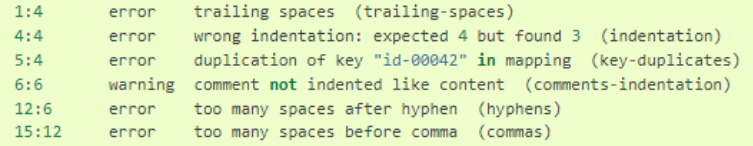
\includegraphics[width=0.8\textwidth]{anexos/Imagens_Blog/diretorio.png}
\fonte{yamllint docs.}
\end{figure}
\FloatBarrier

\textbf{Obs.:} Antes, é legal que você tenha olhado os arquivos das outras equipes que conseguiram validar o equipe.yaml, assim você consegue entender melhor como é a estrutura do arquivo. Se preferir baixar o nosso, é só acessar \href{https://svn.spo.ifsp.edu.br/svn/a6pgp//A2022-PDS-SEG/Bunka_Bytes/equipe.yaml}{aqui}, mas também olhe lá no \href{https://dicas.ivanfm.com/aulas/blogs-de-trabalhos.html}{Blog de Trabalhos} os que já estão validados (é só clicar no \textit{link} chamado "\acs{svn}" dos projetos).

Para entender melhor essas mensagens, recomendo que leia também as regras dispostas na documentação do \gls{Yamllint}, lá você vai encontrar o que significa cada erro/\textit{warning} gerado nesse \textit{log}, além de situações em que a estrutura disposta falhe ou passe nos testes. Porém, existem alguns erros comuns que pode ser que você se confunda mais caso leia a documentação. Alguns deles são:

\begin{itemize}
    \item \textbf{Erro - Trailling spaces:} esse erro acontece quando você não remove o espaço depois da última palavra de uma linha. Por isso, fique atento aos números a direita do \textit{log}, eles mostram em qual linha está aquele erro. O cursor precisaria estar "colado" no número 2 para que não apontasse o erro de \textit{trailling spaces} Por exemplo:
        \begin{figure}[htb]
        \centering
        \caption{Erro - \textit{Trailling spaces}}
        
\includegraphics[width=0.4\textwidth]{anexos/Imagens_Blog/erro1.png}
        \fonte{Os autores.}
        \end{figure}
        \FloatBarrier
    
    \item \textbf{Erro - no new line at the end of file: } nesse caso você precisa se certificar de que a última linha do seu arquivo é uma linha em branco. Aqui percebemos que a linha 15 é a última linha do arquivo que está em branco. Dessa maneira:
    \begin{figure}[htb]
        \centering
        \caption{Erro - \textit{no new line at the end of file}}
        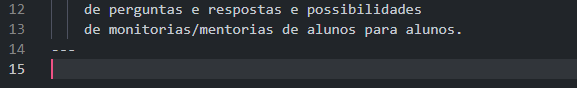
\includegraphics[width=0.4\textwidth]{anexos/Imagens_Blog/erro2.png}
        \fonte{Os autores.}
        \end{figure}
        \FloatBarrier
    
    \item \textbf{Erro - line too long (X > 80 characters):}  esse erro indica que as linhas de um arquivo .yaml não podem ter mais do 80 caracteres, então se você se deparar com ele, quer dizer que no lugar do "X" estará a quantidade de caracteres daquela linha, sendo essa maior do que 80. Uma dica para isso é quebrar as linhas do texto dando alguns espaços aqui e ali, e não fazer um texto corrido de uma vez (mas cuidado com as monografias).
    
    \item \textbf{Erro - found character '$\backslash$t' that cannot start any token (syntax):} aqui você deve se lembrar lá de cima quando falei sobre a formatação do arquivo, pois esse erro é devido ao uso de tabulação em alguma linha do seu equipe.yaml. 
\end{itemize}

\textbf{Dicas extras e considerações finais}
Uma coisa muito importante a se atentar é o cuidado com os caracteres especiais, pois pode ser que seu arquivo lá no \acs{svn} apareça de um jeito estranho, mais ou menos assim:

\begin{figure}[htb]
        \centering
        \caption{Cuidado}
        
\includegraphics[width=0.7\textwidth]{anexos/Imagens_Blog/cuidados.png}
        \fonte{Os autores.}
        \end{figure}
        \FloatBarrier

Isso geralmente acontece pelo \textit{Unicode} do seu arquivo não ser \textbf{UTF-8}. Por isso, ao salvar o arquivo, verifique se a codificação dele está no padrão esperado.

Outra coisa importante de se saber é se \textbf{seu arquivo só vai ser atualizado na página do Dicas Ivan, quando o site for recompilado, o que ocorre a cada dois dias}. Então, fique tranquilo se a atualização não for imediata: é normal. 

Uma dica é sempre verificar o \textit{log} do equipes.yaml, para ver quando/se a compilação já foi feita. Aliás, lá você vai perceber o mesmo tipo de validação que ocorre no \gls{Yamllint}, pois os arquivos que não foram compilados possuem seus erros logo abaixo.

Por último, não esqueça: o Google é seu amigo, se não encontrar algum erro super estranho na documentação, copie-o e cole-o no Google, pode ser que com um pouquinho de garimpo, você encontre a solução que procura.

Por hoje é isso pessoal, se tivermos mais dicas e relacionados para compartilhar com vocês, fiquem atentos nas próximas postagens.

Até mais! :) 

\textbf{Fontes:}

\noindent\href{https://pt.stackoverflow.com/questions/330821/o-que-significa-executar-lint-no-código}{https://pt.stackoverflow.com/questions/330821/o-que-significa-executar-lint-no-código}

\noindent\href{https://yamllint.readthedocs.io/en/stable/}{https://yamllint.readthedocs.io/en/stable/}

\noindent\href{https://www.redhat.com/pt-br/topics/automation/what-is-configuration-management}{https://www.redhat.com/pt-br/topics/automation/what-is-configuration-management}

\noindent\href{https://www.redhat.com/pt-br/topics/automation/what-is-yaml}{https://www.redhat.com/pt-br/topics/automation/what-is-yaml}

\section{Gerando o Vídeo do Gource}
Olá, Bunkers!\\
Estamos aqui hoje com a missão de ajudar vocês a gerar o vídeo no famoso \gls{gource}. Nosso objetivo principal com este \textit{post} é compilar o máximo de informações possíveis de forma simples e objetiva em um único lugar para que vocês não precisem ficar garimpando pedacinhos de informação em diversos \textit{sites} para cumprir uma tarefa que não é difícil.

\textbf{Primeiramente, o que é o Gource?}

O \gls{gource}, nada mais é do que uma ferramenta que permite visualizar o desenvolvimento de um \textit{software} a partir dos \textit{commits} realizados em um repositório (no nosso caso o \acs{svn}) criando um gráfico em formato de árvore.
Um dos requisitos da disciplina de \acs{pds} é que a cada \underline{bimestre, entrega e apresentação feita}, deve ser publicado no canal do YouTube da equipe o vídeo gerado no Gource. 

Segundo a \href{https://dicas.ivanfm.com/programacao/scm/controle-de-versao/gource.html}{bíblia do Ivan}, o vídeo do \gls{gource} deve cumprir as seguintes configurações:
\begin{itemize}
    \item Alterar os userid do repositório por nomes dos participantes;
    \item Colocar uma imagem distinta e especifica para cada usuário;
    \item Utilizar opção \textbf{–key};
    \item Utilizar as opções de \textit{caption} para registrar as principais mudanças feitas no repositório;
    \item Os vídeos devem ter no máximo 1 minuto para cada bimestre; 
\end{itemize}

\textbf{Borá lá trabalhar}

\textbf{1. Instalação}

Para instalar o \gls{gource} é só clicar \href{https://github.com/acaudwell/Gource/releases/download/gource-0.47/gource-0.47.win64-setup.exe}{aqui} (pode confiar que não é vírus).

Use \href{https://www.youtube.com/watch?v=WMEyeu1FKhw}{este tutorial} encontrado no \gls{youtube} para instalar o \textit{ffmpeg}, ele serve para converter o vídeo em .mp4, vamos entender isso melhor mais pra frente.

\textbf{Dica:} É importante que você verifique se as variáveis de ambiente estão devidamente configuradas, caso contrário o terminal irá reclamar quando você começar a rodar os comandos.\\

\textbf{2. Testando 1,2,3}

Clone o repositório \acs{svn} da sua equipe e cole na área de trabalho ou em uma pasta de fácil acesso, faça o passo a passo localmente, nunca dentro do repositório oficial da disciplina.

Abra o terminal local ou cmd: para isso, aperte SHIFT + Botão direito do mouse e vá até a opção "Abrir o PowerShell aqui" ou "Abrir janela de comando aqui".

\begin{figure}[htb]
        \centering
        \caption{Exemplo de como abrir o terminal}
        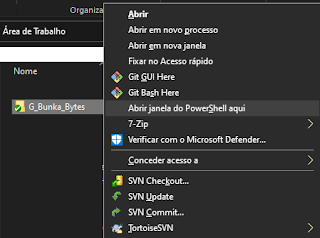
\includegraphics[width=0.4\textwidth]{anexos/Imagens_Blog/exemplo_abrir_terminal.png}
        \fonte{Os autores.}
        \end{figure}
        \FloatBarrier

Digite \textbf{gource} e aperte Enter

Apareceu um vídeozinho?????? 

Boooa, o \gls{gource} foi instalado corretamente, mas como alegria de Ifiano dura pouco, aperte ESC para sair pois ainda faltam os requisitos da bíblia.\\

\textbf{3. Alterando o log}

Vamos precisar criar um log, para isso execute o seguinte comando usando o nome da sua equipe:
\lstset{language=Fortran,
             basicstyle=\ttfamily\small,
             showstringspaces=false
    }
        \begin{lstlisting} 
            --output-custom-log BunkaBytes
        \end{lstlisting}
        
Após executar o comando, volte na pasta clonada e veja que um arquivo foi criado.

\begin{figure}[htb]
        \centering
        \caption{Arquivo de caption}
        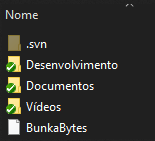
\includegraphics[width=0.3\textwidth]{anexos/Imagens_Blog/arquivo_log.png}
        \fonte{Os autores.}
        \end{figure}
        \FloatBarrier

Abra este arquivo em um editor de texto de sua preferência e altere o prontuário correspondente a cada componente da equipe por seu primeiro nome, então vamos disso:

\noindent 1649709679|sp1234567|A|/A2022-PDS-SEG/Bunka\_Bytes/Documentos/AnaliseProjetos.pdf \\
\noindent 1649709679|sp7654321|A|/A2022-PDS-SEG/Bunka\_Bytes/Documento/PropostaInicial.pdf

Para isso:

\noindent 1649709679|Anai|A|/A2022-PDS-SEG/Bunka\_Bytes/Documentos/AnaliseProjetos.pdf \\
\noindent 1649709679|Jose|A|/A2022-PDS-SEG/Bunka\_Bytes/Documento/PropostaInicial.pdf

\textbf{Dica:} No bloco de notas padrão do \textbf{Windows}, use o Ctrl+H para localizar e substituir as linhas mais rápido.

Não é obrigatório, mas para você que prefere ir verificando se as coisas estão acontecendo certinho conforme estão sendo desenvolvidas, rode o seguinte comando para começar a ver a mágica acontecendo - lembre-se de que é com o nome da sua equipe:

\lstset{language=Fortran,
             basicstyle=\ttfamily\small,
             showstringspaces=false
    }
        \begin{lstlisting} 
            gource BunkaBytes
        \end{lstlisting}
        
\textbf{4. Colocando vossos belos rostos no vídeo}

Crie uma pasta "Imagens", "Avatares" ou algo do tipo dentro do seu repositório clonado e coloque dentro dela uma foto correspondente a cada membro da equipe, recomendamos que utilizem o formato png ou jpeg. O nome da imagem deve ser idêntico ao nome que foi inserido anteriormente no \textit{log}. 

Execute o seguinte código para verificar se funcionou:

\lstset{language=Fortran,
             basicstyle=\ttfamily\small,
             showstringspaces=false
    }
        \begin{lstlisting} 
    gource --output-custom-log BunkaBytes --key --user-dir Imagens
        \end{lstlisting}

\textbf{5. Criando o Caption}

Crie um arquivo de \textit{caption}, nele deve constar os \textit{commits} mais importantes dos que estão no \textit{log}, porém ao invés do nome do arquivo, após o pipe ( | ) descreva o que foi feito, exemplo:

\noindent 1651981117|Jose|M|/A2022-PDS-SEG/Bunka\_Bytes/Desenvolvimento \\

\textbf{6. Gerando o vídeo}

Não existe um tempo padrão ou pré-definido pelo \gls{gource}, o ideal é você utilizar as \textit{flags} e ir testando, as que utilizamos são:

\begin{itemize}
    \item \textbf{--caption-duration 5}: define o tempo para cada caption;
    \item \textbf{--max-file-lag 5}: define o tempo máximo para cada caption; 
\end{itemize}

Para gerar o vídeo em si, nós basicamente vamos juntar todos os comandos e \textit{flags} já citados aqui, ficando mais ou menos assim:

\lstset{language=Fortran,
             basicstyle=\ttfamily\small,
             showstringspaces=false
    }
        \begin{lstlisting} 
    gource BunkaBytes --key --user-image-dir Imagens --caption-file 
    caption --caption-duration 5 --max-file-flag 5 -o gource.ppm 
        \end{lstlisting}
  
textbf{Atenção:}  veja o vídeo rodando até o final, espere que a janela feche automaticamente, caso você pressione ESC e saia antes da execução terminar, o vídeo será gerado até aquele momento apenas.\\

\textbf{7. Convertendo para mp4}

Aqui entra a parte do \textit{ffmpeg}, é fundamental que ele esteja instalado e com as variáveis de ambiente devidamente configuradas, caso contrário não irá funcionar. Mas se tudo estiver certinho basta digitar o seguinte comando:

\lstset{language=Fortran,
             basicstyle=\ttfamily\small,
             showstringspaces=false
    }
        \begin{lstlisting} 
 ffmpeg -y -r 60 -f image2pipe -vcodec ppm -i gource.ppm -vcodec 
 libx264 -preset medium -pix_fmt yuv420p -crf 1 -threads 0 -bf 0 
 gource.mp4
        \end{lstlisting} 

\textbf{8. Conclusão}

Volte até a pasta e veja que o vídeo estará convertido em .mp4 e você pode visualiza-lo com qualquer reprodutor de vídeo.

E prontinho! o vídeo está pronto e já pode ser publicado no \gls{youtube}. \\

\textbf{Avisos:}
\begin{itemize}
    \item Este tutorialzinho está direcionado aos usuários de Windows, pois foi neste sistema operacional que geramos o vídeo. 
    \item A cada bimestre apenas dê um: \textbf{SVN Update} na pasta, altere o caption e continue gerando o vídeo normalmente.
    \item Acesse nosso canal no \href{https://www.youtube.com/channel/UCOJVZlclPTqngZQwPS9Fvpg/featured}{YouTube} para ver nossos vídeos do \gls{gource} como exemplo.
\end{itemize}

\textbf{Fontes:}

\noindent\href{https://aneisiata.blogspot.com/2019/04/gource.html}{https://aneisiata.blogspot.com/2019/04/gource.html}

\noindent\href{https://blog.dyegomaas.com.br/posts/artigo-como-visualizar-desenvolvimento-com-gource/}{https://blog.dyegomaas.com.br/posts/artigo-como-visualizar-desenvolvimento-com-gource/}

\noindent\href{https://thiagogomesverissimo.github.io/posts/gource-organization}{https://thiagogomesverissimo.github.io/posts/gource-organization}


\section{11\textordfeminine \, Semana - 23/05 à 29/05}
Estamos de volta, Bunkers!

Visto que nesta semana ocorreram os conselhos de classe nós não tivemos aula em alguns dias e em outros apenas de forma remota ou com carga reduzida, nós conseguimos focar um pouco mais no projeto realizando ajustes na aplicação e documentação conforme haviam sido levantados por nós e pelos professores a partir das entregas do bimestre e da \acs{POC}.

Decidimos então que durante essa semana trabalharíamos nestes ajustes e para a próxima iniciaremos uma nova \gls{Sprint}, trabalhando em outras histórias de usuário dos épicos de Gestão de Perguntas e Gestão de Respostas, além de finalizar a história de autenticação de usuários e iniciar o épico de Gestão de Eventos, visando a próxima entrega que já seria uma versão inicial do projeto. 

Falando sobre os ajustes na documentação, adicionamos o \gls{heroku} no desenho da arquitetura, criamos uma sessão para descartes/mudanças, criamos os \textit{QR Codes} dos \textit{links} do \textit{deploy} e enviamos o código inicial da documentação no \gls{svn}. 

No \gls{front-end} da aplicação, confirmamos a criptografia e passamos as URLs para análise no SSLabs (o \gls{front-end} recebeu notas A e a \acs{api}, notas A+), arrumamos o \textit{deploy} da aplicação Web (estudando também novas plataformas para ter um plano B), ajustamos as rotas do \textit{react-router-dom}, adicionamos as requisições da \acs{api} e o \textit{redux}. Já no \gls{back-end}, foi adicionado o cadastro de \textit{tag}, a busca de perguntas por id, verificações de usuário para algumas requisições, implementação do cargo de administrador na \acs{api}, totalizador de curtidas na pergunta e de respostas na pergunta, além da inclusão dos primeiros testes unitários. Foram alteradas as \acs{uri} das requisições e a \acs{api} agora faz uso do \textit{Swagger} 3 para a documentação, com autenticação na própria interface.

As tarefas realizadas por cada componente da equipe durante a semana foram:
\begin{itemize}
    \item Anai e Julia - Realizaram os ajustes e configurações na documentação.
    \item Jamilli - Arrumou o deploy da aplicação Web, ajustou as rotas e iniciou a captura de \textit{token} de usuário via \acs{jwt}.
    \item José - Adicionou as requisições faltantes da \acs{api} no \gls{front-end} e o \textit{redux}.
    \item Kaiky - Adicionou os ajustes e alterações no \gls{back-end} e banco de dados. 
\end{itemize}

\textbf{Por: Julia Romualdo}

\section{12\textordfeminine \, Semana - 30/05 à 05/06}
Estamos de volta, Bunkers!

Nesta semana, como previsto, demos início a uma nova \gls{Sprint} para iniciar a história de usuário de Autenticação de Usuários e finalizar os épicos de Gestão de Perguntas e Respostas, principalmente na parte do \gls{front-end}, visto que para a \gls{POC} demos mais atenção a nossa \acs{api} - que já possui todos os \textit{endpoints} esperados para estes épicos, passando apenas por alguns ajustes conforme novas necessidades foram surgindo. Entretanto, não conseguimos nos reunir durante a semana para discutirmos o andamento das tarefas em conjunto de forma síncrona/presencial, mas, além de termos falado mais de forma assíncrona, aproveitamos a aula de segunda-feira para conversarmos sobre o andamento do projeto e sanar as dúvidas pendentes com os professores, não somente sobre a aplicação, mas também sobre a documentação - visto que recebemos também o \textit{feedback} sobre a documentação da \acs{POC}. Dessa forma, as tarefas foram ficando mais claras para que continuássemos com a mão na massa ao longo da semana, já que no mesmo dia definimos quais eram as prioridades faltantes e depois fomos apenas atualizando conforme o decorrer dos dias.

As tarefas realizadas por cada membro da equipe ficaram da seguinte forma:
\begin{itemize}
    \item Anai - Ajustou a documentação para a entrega da primeira versão.
    \item Jamilli - Adicionou autenticação no \gls{front-end}, ajustou alguns erros e melhorou a parte visual.
    \item José - Alterou requisições para compatibilidade com a \acs{api} e iniciou a funcionalidade de busca de perguntas.
    \item Julia - Estudou como gerar as métricas do StatSVN e iniciou os testes relacionados.
    \item Kaiky - Modelou o diagrama de classes e fez os ajustes necessários na \acs{api}. 
\end{itemize}

\noindent Para a próxima semana, pretendemos finalizar o que faltar no desenvolvimento da aplicação para a primeira entrega, assim como os documentos e a apresentação necessária.

\textbf{Por: Julia Romualdo}

\section{13\textordfeminine \, Semana - 06/06 à 12/06}
Estamos de volta, Bunkers!

Nesta semana, nós demos continuidade a \gls{Sprint} de desenvolvimento dos épicos de Gestão de Respostas e Gestão de Perguntas, além da autenticação de usuário, e fizemos bastante progresso no estabelecimento das conexões da \acs{api}, no entanto, deixamos muitas tarefas para o final de semana e percebemos que vamos precisar de mais uma \gls{Sprint} para conseguir finalizar tudo com todos os ajustes que nos propomos. Temos a aplicação funcionando bem, porém precisamos finalizar detalhes importantes para a usabilidade. Com relação a \acs{api}, estamos bem encaminhados, inclusive na parte de testes, pois conseguimos incluir a biblioteca \acs{jacoco} para cobertura de testes. No final, nosso maior inimigo tem sido o tempo, visto que também precisamos documentar algumas coisas da aplicação antes da primeira entrega.

No momento de aula, conversamos sobre o funcionamento e falhas que estavam havendo na comunicação da equipe, fomos orientados com relação ao que seria avaliado e a partir disso, definimos os tópicos que seriam abordados na apresentação e as prioridades para desenvolvimento, pois com muitas tarefas e pouco tempo é importante que todos saibam o que é essencial para a entrega.

Como temos tido dificuldade em nos reunimos presencialmente, decidimos que aproveitaremos melhor os momentos em sala de aula que estaremos juntos - e com os professores por perto - para tirar dúvidas e definir as tarefas que serão realizadas no restante da semana e também, pelo mesmo motivo, priorizaremos a comunicação assíncrona da equipe, principalmente pelo \gls{WhatsApp}, mandando resumos do que foi feito por cada um durante a semana, dessa forma garantimos também que todos saibam o que está acontecendo em cada parte do projeto.

As tarefas realizadas por cada membro da equipe foram organizados da seguinte maneira:
\begin{itemize}
    \item Anai - Trabalhou na documentação visando a próxima entrega, ajustou o protótipo e iniciou a criação dos slides para a apresentação. 
    \item Jamilli - Arrumou o problema do \acs{cors}, refatorou códigos e ajustou o \acs{css} e iniciou a documentação sobre a segurança da aplicação.
    \item José - Refatorou alguns códigos, criou componentes reutilizáveis, ajustou \textit{layout}, corrigiu \textit{bugs} e criou a tela de cadastro.
    \item Julia - Ajustes na documentação e testes na geração das métricas no \gls{statsvn}.
    \item Kaiky - Terminou os testes unitários de Pergunta, Adicionou o \acs{jacoco} na \acs{api} para cobrir os testes, arrumou o diagrama de classes, \acs{dtr} e \acs{der} e iniciou a documentação do plano de testes.
\end{itemize}

Na quinta-feira (09/06), a diretoria do campus comunicou que as aulas estariam suspensas até o dia 19/06 por conta do crescimento do número de casos de Covid-19 entre alunos e servidores, então a apresentação da primeira versão aconteceria de forma remota, no mesmo dia previsto (13/06). Entretanto com muita argumentação e com os deuses da programação a nosso favor, os professores concordaram em deixar as apresentações e as entregas para o dia 20/06 quando retornarmos ao formato presencial, com isto nosso objetivo para a próxima semana é continuar desenvolvendo e aprimorando aquilo que foi proposto para a entrega. 

\textbf{Por: Julia Romualdo}

\section{14\textordfeminine \, Semana - 13/06 à 19/06}
Estamos de volta, Bunkers!

Nesta semana, devido ao adiamento da entrega e apresentação da primeira versão na semana passada, pudemos criar uma \gls{Sprint} extra, que tinha como objetivo realizar melhorias do que havia sido proposto na \gls{Sprint} anterior. 
Aproveitamos então para nos reunirmos no início da semana e trabalhar na definição dos atributos do cadastro, como: requisitos de senha e quais domínios de \textit{e-mails} estariam disponíveis para seleção. Começamos também, a pensar em métodos e abordagens para aplicarmos planos de testes e usabilidade em um futuro próximo, com objetivo de validar com os \gls{friend}'s - como chamamos os usuários do \gls{ifriends} - se nosso sistema está intuitivo para uso. Ainda neste momento de reunião, aproveitamos para tirar uma tarefa pendente do caminho e gravamos o vídeo com relação a \acs{POC}. 
Com todos sabendo suas tarefas e o que tinha que ser feito, partimos para a execução durante a semana, mantendo a comunicação assíncrona via \gls{WhatsApp}.

No \gls{front-end} da aplicação, trabalhamos no \textit{feedback} visual, padronização e validação de campos no \textit{login} e no cadastro, internacionalização, menu superior com mais opções (como os dados do usuário logado, botão de internacionalização e \textit{logout}), \textit{timeout} na sessão para verificar expiração do \textit{token}, tratamento e captura de erros da \acs{api} com mensagens, além das rotas que foram ajustadas de modo que o \gls{friend} já logado não possa acessar as telas de \textit{login} e cadastro. Além disso, também foi feito um teste inicial com a hospedagem de imagens via \acs{api} do \gls{imgbb}.

No \gls{back-end}, os \textit{bugs} de atualização da pergunta forma ajustados, uma requisição para devolver as categorias foram criadas, os testes do \textit{service} da categoria foram feitos, a segurança da \acs{api} obteve nota A+ e criou-se a tabela "curso" no banco de dados.

Esta semana todos precisaram escrever um pouco na documentação, pois os pontos do desenvolvimento como testes, novas tecnologias e segurança, precisavam ser documentados. Entretanto, especificamente na estrutura da documentação, nós atualizamos os \textit{posts} do \textit{blog}, atas das reuniões e a modelagem do banco de dados (\acs{der}, \acs{dtr} e \acs{dd}). Com base no \textit{feedback} dos professores na documentação da \acs{POC},  melhoramos a introdução, de forma que ela ficasse mais aprofundada na temática do projeto. Adicionamos uma tabela de métricas do desenvolvimento geral do projeto, já que estamos com dificuldade e não conseguimos gerar as métricas no \gls{statsvn}, criamos também a sessão de análise de concorrência para compararmos o \gls{ifriends} com o \gls{moodle} e \gls{scoold} e por último, cuidamos dos apêndices, movendo para lá a prototipagem, dicionário de dados, histórias de usuários e documentos anteriores.

Cada componente da equipe realizou as seguintes atividades durante a semana:

\begin{itemize}
    \item Anai - Criou a sessão de análise da concorrência, cuidou dos apêndices e montou o \textit{layout} dos slides da apresentação.  
    \item Jamilli - Traduziu dos textos para  a internacionalização, fez ícone do usuário no menu ter mais ações, implementou \textit{timeout} na sessão do usuário, a tratou erros das requisições vindas \acs{api} e os redirecionamento das rotas.
    \item José - \textit{Feedback} visual, padronização e validação de campos, tela de cadastro, inclusão de uma \acs{api} para salvar imagens na nuvem e configuração da internacionalização.  
    \item Julia - Atualização \textit{posts blog}, atas das reuniões e modelagem de dados, melhoria da introdução e criação da tabela de métricas de desenvolvimento do projeto.
    \item Kaiky - Arrumou os \textit{bugs} da pergunta, fez a requisição para devolver as categorias criadas, os testes do \textit{service} da categoria, a segurança da \acs{api}, ajustes no banco e modelagem de dados. 
\end{itemize}

Nós e as outras equipes da turma estamos enfrentando um problema desde sábado de manhã (18/06), que é a queda do \gls{svn}, sem ele nós não estamos conseguindo \textit{commitar} as coisas que estamos terminando e nem puxar os dados que estão no repositório para preencher a tabela de métricas e gerar o vídeo do \gls{gource}. Por isso, estamos nos virando com um \textit{backup} que fizemos no \gls{github} e tentando puxar as novas mudanças de cada um para a versão final.

Para a próxima semana temos como objetivo apresentar a primeira versão e realizar a reunião retrospectiva da entrega. 

\textbf{Por: Julia Romualdo}